\chapter{Exceptions}
\subsection{Raising exceptions intraprocedurally}
As it has not been our primary goal to fully support exception handling, but only to support some kind of simple exception handling in order to be able to handle the magic method \inlinecode{\_\_getattr\_\_}, we have only concentrated on except blocks (catch blocks) without types that catches all raised exceptions. In particular we don't support except blocks like \inlinecode{except AttributeError as e}.

As a consequence the changes to our type analyzer has been minor. When an exception is possibly raised the type analyzer writes that particular exception object to a special temporary variable where we store the latest raised exception. If the exception is raised by means of a \inlinecode{RaiseNode} in the CFG, the exception object will already be stored in a temporary variable. This is the case because the code \inlinecode{raise Exception()} is represented as follows in our CFG:

\begin{listing}[H]
	\begin{center}
		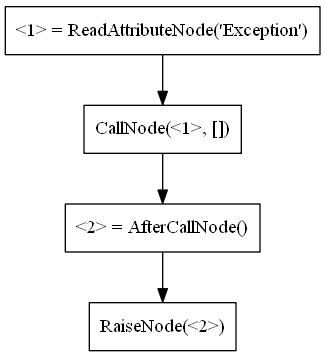
\includegraphics[width=0.4\textwidth]{images/raiseexception.png}
	\end{center}
	\vspace{-20pt}
\end{listing}

Therefore, our type analyzer can just take that object (for the example: the object in \inlinecode{<2>}) an store it in the temporary exception variable.

When an exception is not raised by means of a \inlinecode{RaiseNode}, our type analyzer creates a new exception object on its own. If for instance an attribute is read on an object without that attribute, we create a new \inlinecode{AttributeError} object and store it on the heap in our lattice. We do this as follows:

\begin{enumerate}
	\item The \inlinecode{\_\_builtin\_\_} module object on the heap is looked up,
	\item The attribute "AttributeError" is looked up on the \inlinecode{\_\_builtin\_\_} object from (1); this should always yield a \inlinecode{NewStyleClassObjectLabel},
	\item We manually create an instance of that particular class label found in (2), stores it on the heap of our lattice and finally also in the temporary exception variable on our stack lattice.
\end{enumerate}


\subsection{Raising exceptions interprocedurally}
The above outline only specifies how we raise exception intraprocedurally, since we so far haven't specified any exception edges in our CFG going across function definitions.

We take care of exceptions interprocedurally by introducing a new type of node for function exit: \inlinecode{ExceptionalExitNode}. Thus for each function we have two exit nodes. We now take each of the CFG nodes of the function that does not have an outgoing exception edge\inlinecode{If a CFG node in a function already has an outgoing exception edge, it is because it is inside a try-except block.} and connect them to the exceptional exit node by an exception edge.

Recall from the section about functions, that we upon a call to a function update the call graph with call edges from the call node to the entry node of the function, and from the exit node of the function to the after call node. In order to accomodate exceptions interprocedural we now also add a \textit{call exception edge} from the exceptional exit node of the function to the except block of the call node. To illustrate this consider the below example together with its corresponding (partial) CFG:

\begin{listing}[H]
	\begin{minted}[linenos]{python}
class C(object):
  if (trickyComputation()):
    a = 42
x = C()
def foo():
  result = x.a
  return result
try:
  y = foo()
except:
  err = "An error occured"
	\end{minted}
\end{listing}

\begin{listing}[H]
	\begin{center}
		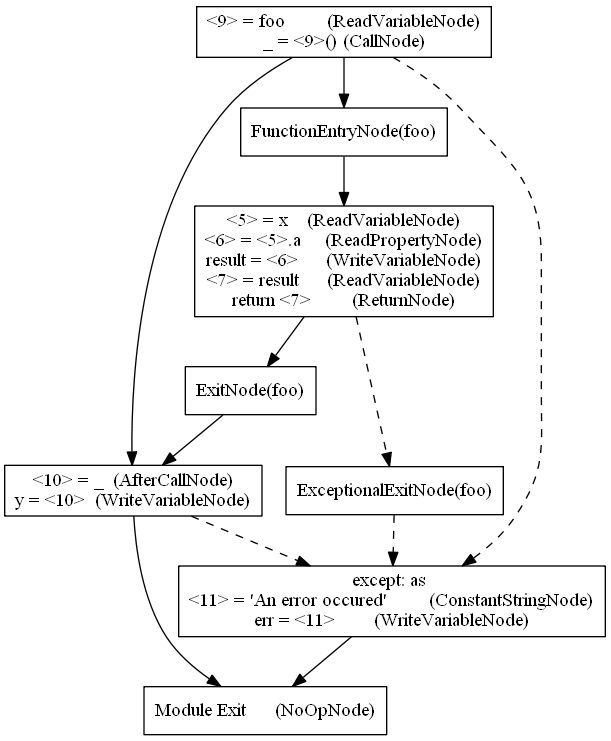
\includegraphics[width=0.75\textwidth]{images/exception1.png}
	\end{center}
	\vspace{-10pt}
\end{listing}


\subsection{Catching exceptions}
The constraint function for an \inlinecode{ExceptNode} in the CFG reads the value of the temporary variable associated with the latest raised exception. If the exception variable is bottom the solution of this node is simply set to the bottom element of the $State$ lattice. This indicates that the path is infeasible and acts as a simple sort of path sensivity. If the exception variable is actually set to an object on the heap, we just clear the exception variable on the stack by setting it to the bottom element of the $Value$ lattice. Now, the CFG nodes in the except block will change the solution as it looked like when an exception was raised, and the node following the try and except blocks will join the state coming from the try and except block, respectively.

As an example consider the following code:

\begin{listing}[H]
	\begin{minted}[linenos]{python}
class C(object):
  if (trickyComputation()):
    a = 42

x = C()
try:
  y = x.a
  z = "trickyComputation() was true"
except:
  err = "An error occured"
	\end{minted}
	\caption{An example that involves exceptions together with the solution of our type analyzer (see below).}
\end{listing}

Our type analyzer will for this particular code conclude that for the exit node of the program:

\begin{itemize}
	\item \inlinecode{y} is either undefined or 42
	\item \inlinecode{z} is either undefined or "trickyComputation() was true"
	\item \inlinecode{err} is either undefined or "An error occured"
\end{itemize}

For the state at the last program point in the try block, our type analyzer concludes that:

\todo{Explain why y might be undefined according to the analysis}
\begin{itemize}
	\item \inlinecode{y} is undefined or 42
	\item \inlinecode{z} is "trickyComputation() was true"
\end{itemize}